%%%%%%%%%%%%%%%%%%%%%%%%%%%%%%%%%%%%%%%%%
% Stylish Article
% LaTeX Template
% Version 2.0 (13/4/14)
%
% This template has been downloaded from:
% http://www.LaTeXTemplates.com
%
% Original author:
% Mathias Legrand (legrand.mathias@gmail.com)
%
% License:
% CC BY-NC-SA 3.0 (http://creativecommons.org/licenses/by-nc-sa/3.0/)
%
%%%%%%%%%%%%%%%%%%%%%%%%%%%%%%%%%%%%%%%%%

%----------------------------------------------------------------------------------------
%	PACKAGES AND OTHER DOCUMENT CONFIGURATIONS
%----------------------------------------------------------------------------------------

\documentclass[fleqn,10pt]{SelfArx} % Document font size and equations flushed left

\usepackage{lipsum} % Required to insert dummy text. To be removed otherwise

%----------------------------------------------------------------------------------------
%	COLUMNS
%----------------------------------------------------------------------------------------

\setlength{\columnsep}{0.55cm} % Distance between the two columns of text
\setlength{\fboxrule}{0.75pt} % Width of the border around the abstract

%----------------------------------------------------------------------------------------
%	COLORS
%----------------------------------------------------------------------------------------

\definecolor{color1}{RGB}{0,0,90} % Color of the article title and sections
\definecolor{color2}{RGB}{0,20,20} % Color of the boxes behind the abstract and headings

%----------------------------------------------------------------------------------------
%	HYPERLINKS
%----------------------------------------------------------------------------------------

\usepackage{float}
\usepackage{hyperref} % Required for hyperlinks
\hypersetup{hidelinks,colorlinks,breaklinks=true,urlcolor=color2,citecolor=color1,linkcolor=color1,bookmarksopen=false,pdftitle={Title},pdfauthor={Author}}

%----------------------------------------------------------------------------------------
%	ARTICLE INFORMATION
%----------------------------------------------------------------------------------------

\JournalInfo{2015} % Journal information
\Archive{Research} % Additional notes (e.g. copyright, DOI, review/research article)

\PaperTitle{Password Anomaly Detection} % Article title

\Authors{Mario Murrent} % Authors
%\affiliation{\textsuperscript{1}\textit{Department of Biology, University of Examples, London, United Kingdom}} % Author affiliation
%\affiliation{\textsuperscript{2}\textit{Department of Chemistry, University of Examples, London, United Kingdom}} % Author affiliation
%\affiliation{*\textbf{Corresponding author}: john@smith.com} % Corresponding author

%\Keywords{} % Keywords - if you don't want any simply remove all the text between the curly brackets
%\newcommand{\keywordname}{Keywords} % Defines the keywords heading name

%----------------------------------------------------------------------------------------
%	ABSTRACT
%----------------------------------------------------------------------------------------

%\Abstract{}

%----------------------------------------------------------------------------------------

\begin{document}

\flushbottom % Makes all text pages the same height

\maketitle % Print the title and abstract box

\tableofcontents % Print the contents section

\thispagestyle{empty} % Removes page numbering from the first page

%----------------------------------------------------------------------------------------
%	ARTICLE CONTENTS
%----------------------------------------------------------------------------------------

\section*{Introduction} % The \section*{} command stops section numbering

\addcontentsline{toc}{section}{Introduction} % Adds this section to the table of contents

\paragraph{PassSecure}The purpose is to develop a simple password application which uses machine learning to detect if a password entered by the user is indeed from a genuine user or not. An application to test the selected algorithm is developed and described

%------------------------------------------------

\section{Algorithms}

This section will describe all tested algorithms.

\subsection{Kullback Leibler divergence}
The Kullback Leibler divergence is a non symmetric measure of the difference between two probability distributions P and Q.\cite{kullback} This method will give you a number between 0 and 1, but the problem is that is does not take into account if the password typing speed varies. In fact that algorithm is not suitable for this specific purpose.

\subsection{Manhattan Distance}
The Manhattan distance function computes the distance that would be traveled to get from one data point to the other if a grid-like path is followed. The Manhattan distance between two items is the sum of the differences of their corresponding components\cite{manhattan}.
\newline
The Manhattan distance is according to the paper "Comparing Anomaly-Detection Algorithms for Keystroke Dynamic" \cite{Figueredo:2009dg} on of the best algorithms. 

\section{Implementation Details}
During the training mode all necessary data is collected including:
\begin{itemize}
  \item Total time between first key up and last key up
  \item Total time between first key down and last key down
  \item Time between each key up
  \item Time between each key down
  \item Average key down time
  \item Average key up time
  \item Manhattan distance
\end{itemize}
The complete training consists of a set of training entries. A training entry is only added when the password is correct. Failures are not taken into account. On adding a new training entry the distance to the training set is calculated and the training set is analyzed. Analyzing a training set means recalculating all average values.

\subsection{Used Libraries}
\begin{itemize}
  \item Accord - Image Processing \& Machine Learning Framework (\url{http://accord-framework.net/intro.html})
\end{itemize}

\section{Application}
The application is designed to test the used algorithm to detect if a password entered by the user is indeed from a genuine user or not. It is possible to enter multiple users with specific passwords. Every user is evaluated separately. It is also possible to import or export data which has been recorded.
\begin{figure}[!htb]
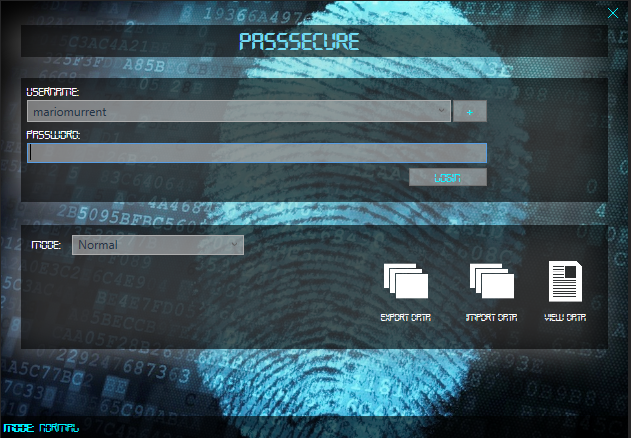
\includegraphics[scale=0.5]{application}
 \caption{A screenshot of applications main window.}
\end{figure}
The data windows is designed to view data which is used for evaluation.
\begin{figure}[!htb]
\includegraphics[scale=0.6]{viewData}
 \caption{A screenshot of the data window.}
\end{figure}
The application has two modes: Training \& Normal. During the training mode all necessary data is collected. In the normal mode the current password is checked against the captured data. A picture on the right side indicates whether the password is accepted or not. Partially accepted means that if might not be the user.
%----------------------------------------------------------------------------------------
%	REFERENCE LIST
%----------------------------------------------------------------------------------------
\phantomsection
\bibliographystyle{unsrt}
\bibliography{sample}

%----------------------------------------------------------------------------------------

\end{document}